
Una buena elección de la tecnología será una condición necesaria, aunque no suficiente, para llevar a cabo un proyecto con éxito.

En este capítulo presentamos las tecnologías utilizadas en el desarrollo de este proyecto. 

\section{Android SDK}
Android  \cite{2}  \cite{3} es un sistema operativo especialmente diseñado para dispositivos móviles. Permite el desarrollo de sus aplicaciones en un lenguaje similar al Java. El sistema operativo nos proporciona de manera sencilla todas las inferfaces para el desarrollo de las aplicaciones que puedan acceder a las funciones del teléfono.\\

\textbf{Android SDK}\\

El SDK de Android ofrece un conjunto de herramientas para el desarrollo de aplicaciones incluyendo:
\begin{itemize}
\item \textbf{Depurador de código}
\item \textbf{Simulador de dispositivos de la plataforma. basado en QEMU}. Siendo QEMU  un emulador de procesadores. 
\item\textbf{ Bibliotecas.}
\item \textbf{Documentación.}
\item \textbf{Ejemplos de código.}

\end{itemize}


\section{Eclipse }


Eclipse es un IDE en Java para
( ver Figura~\ref{fig:eclipse}) para el desarrollo de software. Fue creado por IBM como sucesor de una de sus herramientas y ahora está en manos de la Fundación Eclipse que es quien se encarga de seguir desarrollándolo.
Se decidió usar esta herramienta de desarrollo ya que es totalmente gratuita por lo que no encarece el precio del proyecto y porque el entorno que usamos en Android esta basado en este.  
\begin{figure}[H]
		\centering
		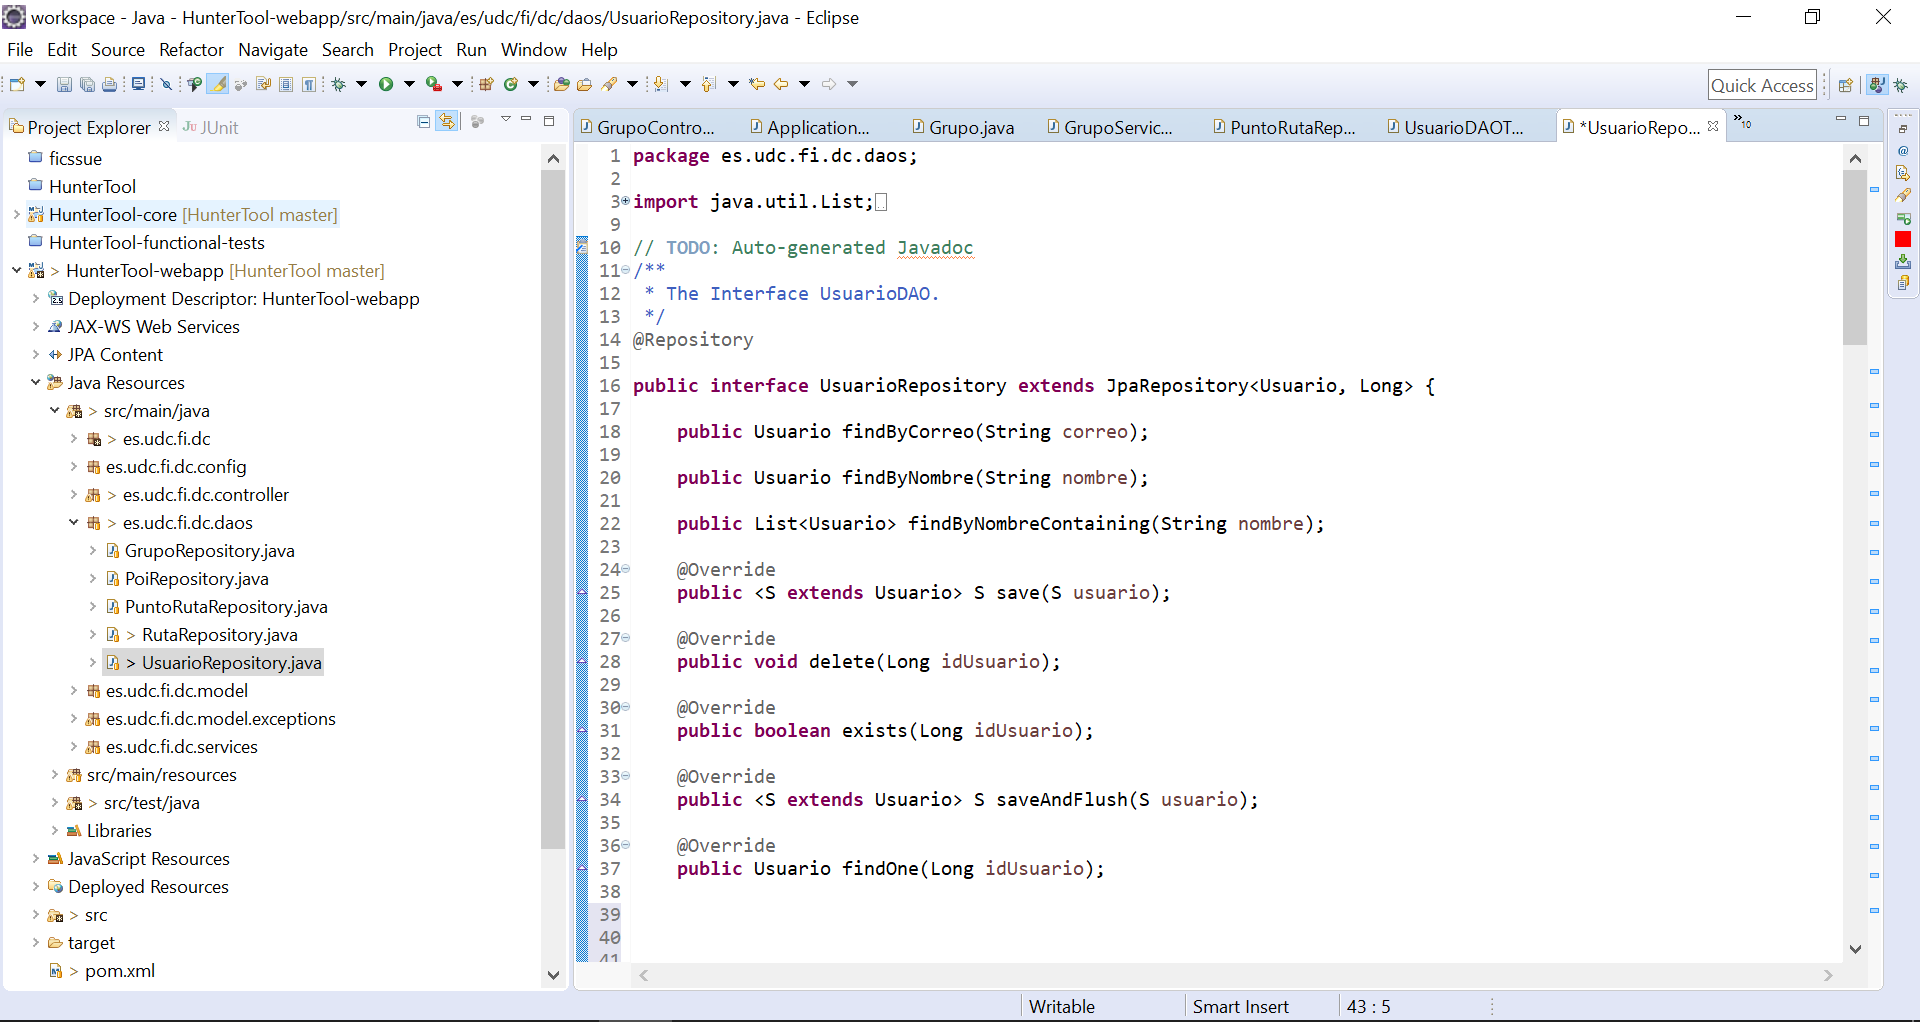
\includegraphics[width=\textwidth] {eclipse.png}
		\caption{Entorno de trabajo Eclipse }
		\label{fig:eclipse}
	\end{figure}
	
	
	
\section{Spring}
Spring es un framework \cite{5} de código abierto que tiene como objetivo ayudar al desarrollador a trabajar con otras APIs de manera más sencilla. Nos proporciona un modelo de programación y configuración integral para aplicaciones empresariales basadas en Java, en cualquier tipo de plataforma de implementación. 
	
Las funcionalidades principales que ofrece son:

\begin{itemize}
\item \textbf{Programación orientada aspectos},es un paradigma que nos ayuda separar aspectos trascendentales del resto del código. Lo que conlleva reducir  la probabilidad de errores en la codificación o ineficiencias.


\item\textbf{ Inyección de dependencias}, patrón que ayuda a reducir el acoplamiento entre los distintos componentes de la aplicación. Esto se consigue haciendo que una entidad externa proporcione a otra sus dependencias y que esta no tenga que crearlas.
Gracias a esto los componentes conocen sus dependencias solamente a traves de un interfaz lo que hace posible que la implementación pueda variar de manera trasparente para estas clases. Código\ref{depen} como ejemplo.




 \begin{lstlisting}[language=java,caption={Inyección de dependencias},label=depen]
@Service
public class GrupoServiceImpl implements GrupoService {

	@Autowired
	GrupoRepository grupoDAO;

	public void setGrupoDAO(GrupoRepository grupoDAO) {
		this.grupoDAO = grupoDAO;
	}


\end{lstlisting} 



\end{itemize}

En el código \ref{depen} se puede ver la anotación @Service y @Autowired. @Service indica que la clase es un componente, concretamente un servicio lo que permite que las clases de implementación sean detectadas automáticamente. @Autowired  permite que se carguen las dependencias de GrupoRepository para poder ser usadas en esta clase.
\section{Android Studio}
Android Studio es el entorno de desarrollo integrado (IDE)  oficial para Android que nos ofrece las herramientas necesarias para crear apps en  dispositivos Android.
Además de ser una potente herramienta para la creación de código permite:

\begin{itemize}
\item Realizar compilaciones  de nuestro código.
\item Renderizado en tiempo real.
\item Soporte para construcción basada en Gradle.
\item Plantillas para crear diseños comunes de Android.
\item Uso de un depurador que te permite depurar apps que se ejecutan en el emulador de Android o en un dispositivo Android.Figura \ref{fig:debug}. Permitiendo:\begin{itemize}
\item Establecer puntos de interrupción.
\item Examinar variables en tiempo de ejecución.
\end{itemize}


\item Generar un APK (Android Application Package) para la ejecución de nuestra aplicación móvil tanto de forma simulada, ayudándonos del simulador que nos proporciona o usando un móvil.(Figura \ref{fig:emulador})
\end{itemize}
\begin{figure}
		\centering
		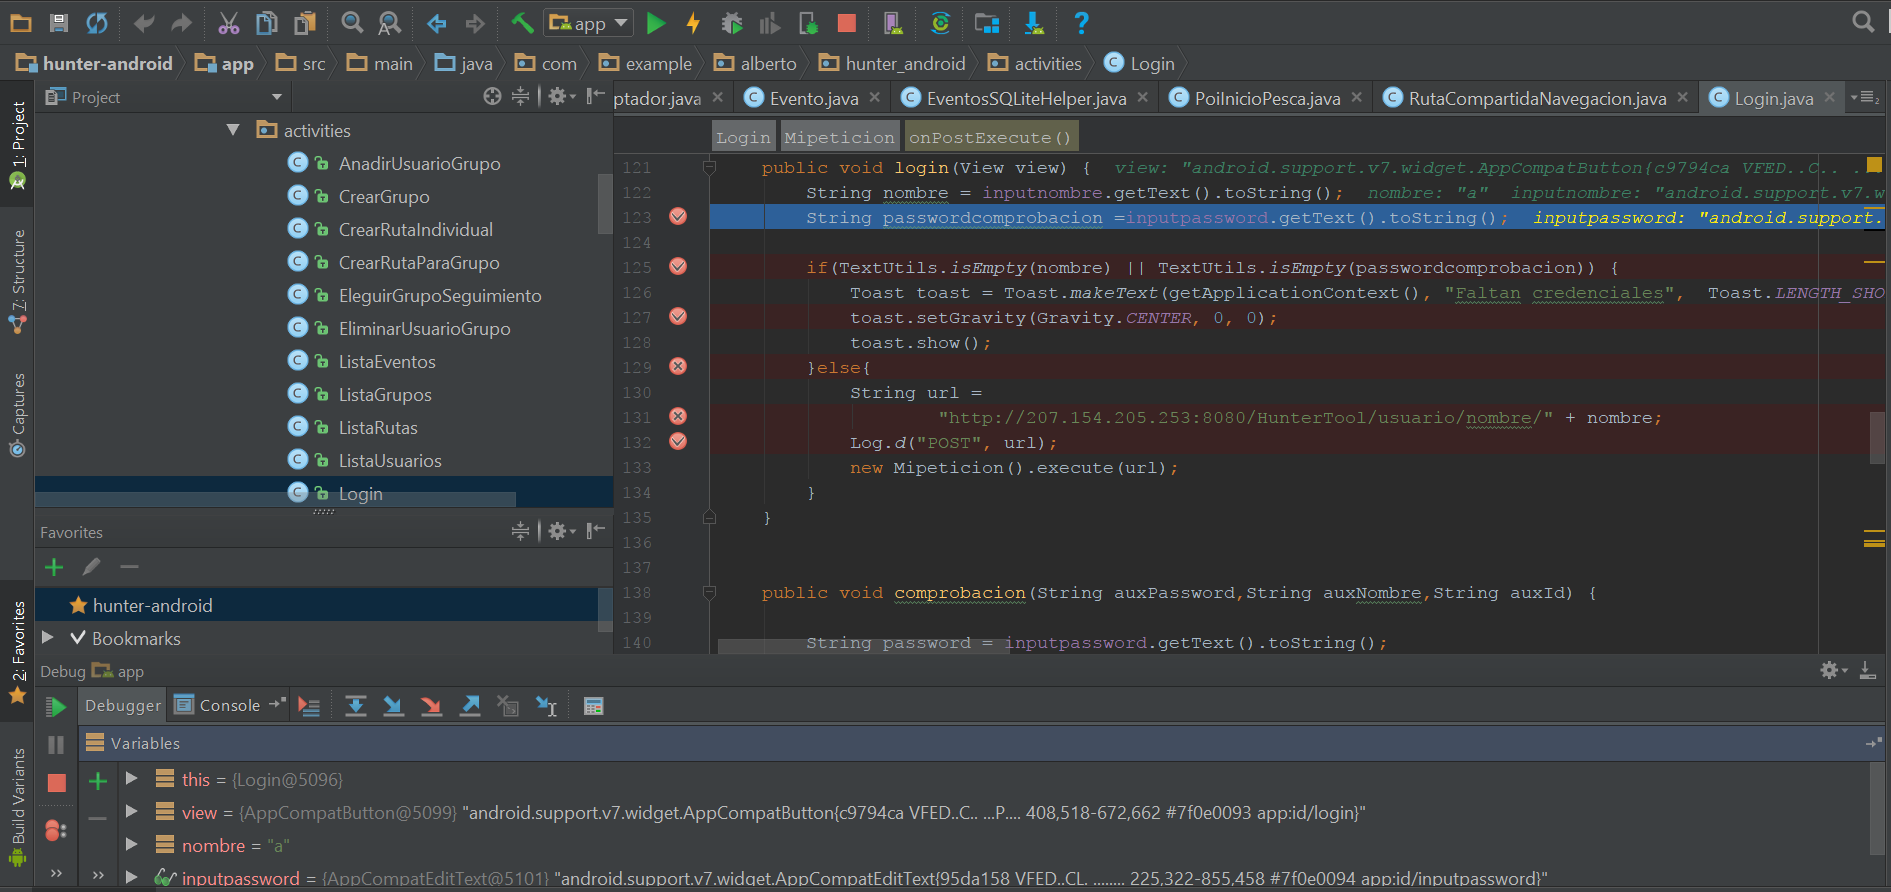
\includegraphics[width=\textwidth] {debug.png}
		\caption{Captura de pantalla realizando app debug }\label{fig:debug}
	\end{figure}
\begin{figure}
		\centering
		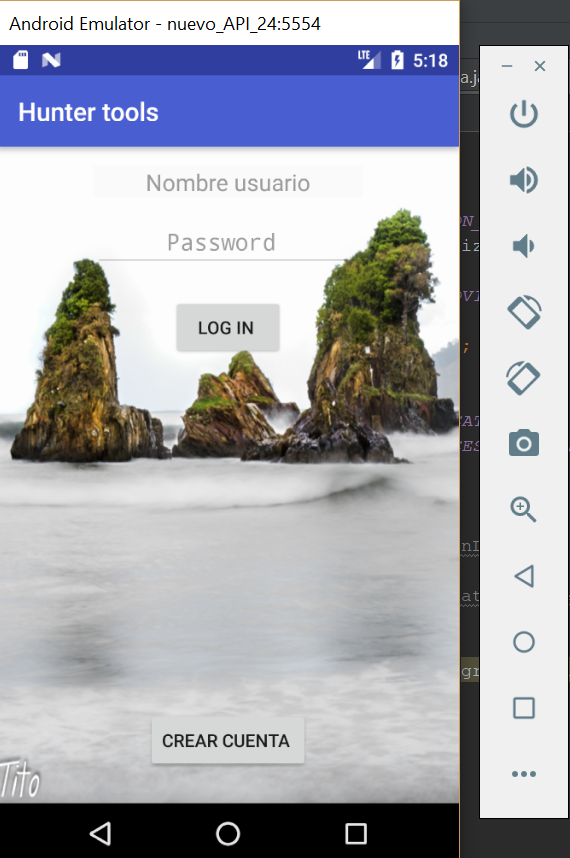
\includegraphics[width=0.6\textwidth] {emulador.png}
		\caption{Emulador de Android con mi aplicación}
		\label{fig:emulador}
	\end{figure}
 



\section{Git}
Git27 es un sistema de control de versiones distribuido. Se trata del gestor de versiones moderno
más empleado y por ello cuenta con una gran comunidad de desarrolladores a su alrededor lo
que favorece la integración de Git con múltiples herramientas.
\section{Maven}
Maven es una herramienta de software para la gestión y construcción de proyectos Java.
 Maven utiliza un Project Object Model (POM) en formato
XML para describir sus dependencias del proyecto. Incluye por defecto con ayudas para la compilación de código o el empaquetado.






\section{Gradle}
Gradle es otra herramienta de software para la gestión, construcción de proyectos y gestor de dependencias. Ofrece
  herramientas de compilación avanzadas, para automatizar y administrar el proceso de compilación, y al mismo tiempo te permite definir configuraciones de compilación personalizadas.



\section{Jackson}

Jackson es parser para el desarrollo de Servicios Web en Java. Implementa un conjunto de   herramientas de procesamiento de datos para Java haciendo que el desarrollo de servicios Rest sean más simples. Se eligió esta opción por lo sencillo que hacia el mapeo de objetos en las peticiones a JSON, transformando  JSON en objetos del dominio y viceversa.








\section{Hibernate}
Hibernate  \cite{4} es una herramienta de mapeo objeto-relacional para la plataforma Java que ayuda a la transformación de objetos del modelo a una entidad de la base de datos persistente. Este mapeo simplifica el trabajo de desarrollo y evita errores en tareas repetitivas.Este mapeo ayuda a  no tener que definir la entidad directamente en nuestro gestor de base de datos. Para conseguir esto debemos usar las anotaciones pertinentes, definir a nivel de base de datos las entidades, restricciones y relaciones. Una vez puestas las anotaciones los accesos a datos de la  bases de datos pasan a ser muy sencillos.





\section{PostgreSQL}
PostgreSQL es SGBD conocido, probado y fiable con un uso muy extendido en la industria. También nos proporciona  el PgAdmin que facilita la gestión y administración de bases de datos ya sea mediante instrucciones SQL o con ayuda de un entorno gráfico. Permite acceder a todas las funcionalidades de la base de datos, consulta, manipulación y gestión de datos.
\section{JUnit}
JUnit es el framework de testing para Java más extendido.
Permite la ejecución de clases Java para evaluar el comportamiento de los métodos a probar.


\vspace{1cm}


